\documentclass[11pt]{article}

\usepackage[margin=1.15in]{geometry}
\usepackage{amsmath}
\usepackage{amssymb}
\usepackage{graphicx}

% The ones vector (1, 1, ..., 1)^T appears throughout; give it one symbol.
\newcommand{\ones}{\mathbf{1}} % the vector of ones, (1, ..., 1)^T
\newcommand{\Cov}{\mathsf{C}}
\newcommand{\Prec}{\mathsf{P}}
\newcommand{\T}{^{\mathsf{T}}}

\title{A correlated prior on galaxy bias across thin redshift bins}
\date{November 2026}
\author{}

\begin{document}

\begin{center}
  {\LARGE A correlated prior on galaxy bias\\[0.3em] across thin redshift bins\par}
  \vspace{1em}
  {\large November 2026\par}
\end{center}
\vspace{1em}

\section{Introduction: why an intermediate bias model}
\label{sec:intro}

A Fisher forecast of galaxy clustering in thin redshift bins must decide
how to parametrize the galaxy bias of each bin.  The bins belong to a few
broad groups: the DESI tracer samples and their chunks, such as BGS,
LRG1, LRG2, LRG3, ELG1 and ELG2.  Within one group the galaxies are
selected the same way, so their biases are expected to be similar but not
identical.

The default model ties all bins of a group to a single amplitude.  If
$D(z)$ is the linear growth factor, normalized to $D(0) = 1$, the tied
model sets
\begin{equation}
  b_i \;=\; \frac{B_g}{D(z_i)},
  \label{eq:tied}
\end{equation}
where $b_i$ is the linear bias of bin $i$, $z_i$ is the bin's redshift,
and $B_g$ is one free amplitude per group $g$.  The $1/D$ evolution keeps
the clustering amplitude $b(z)\,D(z)$ of the group constant, the
behavior measured for DESI-like luminous red galaxies
\cite{Zhou2021}.  It is not the law of a fixed set of galaxies that
follow the flow of matter ("passive evolution"); Section
\ref{sec:conserved} derives that law and the small difference between
the two.

The opposite extreme frees one bias per bin, with flat priors and no
connection between neighbors ("independent").  The dark-energy figure of
merit of the forecast depends on which extreme is chosen, and the
question is how much of it rests on the tying itself.  To answer that,
this note builds the intermediate model: bins may deviate from the
group's trend, but neighboring bins must deviate \emph{together}.

\section{The models}
\label{sec:models}

\subsection{Tied, independent, and correlated biases}
\label{sec:defs}

The model multiplies the tied bias by a fractional deviation
$\delta_i$,
\begin{equation}
  b_i \;=\; \frac{B_g}{D(z_i)}\,\bigl(1 + \delta_i\bigr),
  \label{eq:model}
\end{equation}
with $B_g$ still free (flat prior).  The deviations receive a Gaussian
prior that is correlated inside a group,
\begin{equation}
  \bigl\langle \delta_i\,\delta_j \bigr\rangle
  \;=\; \sigma_b^2\,
  \exp\!\left(-\,\frac{|z_i - z_j|}{L}\right),
  \label{eq:priorkernel}
\end{equation}
and zero across groups.  Here $\sigma_b$ is the prior standard deviation
of a single bin's fractional deviation, and $L$ is the correlation
length in redshift: bins much closer than $L$ deviate almost as one,
bins much farther apart deviate independently.

In the Fisher matrix the convenient parameters are the per-bin
amplitudes
\begin{equation}
  \beta_i \;\equiv\; B_g\,\bigl(1 + \delta_i\bigr),
  \qquad \text{fiducial } \beta_i = B_g,
  \label{eq:beta}
\end{equation}
so that $b_i = \beta_i / D(z_i)$.  Since $\beta_i - B_g = B_g\,\delta_i$,
the prior covariance of the $\beta_i$ within one group is
\begin{equation}
  \Cov \;=\; s^2\,\mathsf{R},
  \qquad
  s \;=\; \sigma_b\,B_g,
  \qquad
  \mathsf{R}_{ij} \;=\; \exp\!\left(-\,\frac{|z_i - z_j|}{L}\right).
  \label{eq:covdef}
\end{equation}
The spread $s$ carries the units of a bias amplitude; the correlation
matrix $\mathsf{R}$ is dimensionless, with ones on the diagonal.

\subsection{What $\sigma_b$ and $L$ mean}
\label{sec:jump}

The kernel of Eq.~\eqref{eq:priorkernel} has two parameters, and they
control two different things.  The diagonal gives the wander of a single
bin,
\begin{equation}
  \mathrm{Var}(\delta_i) \;=\; \sigma_b^2 ,
  \label{eq:wander}
\end{equation}
so $\sigma_b$ sets how far any one bin may drift from the group's
trend $B_g/D(z)$.  The correlation coefficient $r$ of two bins $i$ and $j$ follows from
the same kernel.  By definition,
\begin{equation}
  r \;=\;
  \frac{\langle \delta_i \delta_j \rangle}
       {\sqrt{\langle \delta_i^2 \rangle\,\langle \delta_j^2 \rangle}}
  \;=\;
  \frac{\sigma_b^2\, e^{-\Delta z / L}}{\sigma_b^2}
  \;=\; e^{-\Delta z / L},
  \label{eq:rdef}
\end{equation}
with $\Delta z = |z_i - z_j|$ the bin separation.  The amplitude
$\sigma_b$ cancels: the correlation is set by the separation and $L$
alone.

The jump between two bins now follows from the two pieces above:
with $\mathrm{Var}(\delta_i) = \sigma_b^2$ and
$\mathrm{Cov}(\delta_i, \delta_j) = \sigma_b^2\, e^{-\Delta z / L}$,
the variance of the difference is
$\mathrm{Var}(\delta_i) + \mathrm{Var}(\delta_j)
- 2\,\mathrm{Cov}(\delta_i, \delta_j)$:
\begin{equation}
  \mathrm{Var}(\delta_i - \delta_j)
  \;=\;
  2\,\sigma_b^2\left(1 - e^{-\Delta z / L}\right).
  \label{eq:jumpvar}
\end{equation}
For separations much smaller than the correlation length,
$\Delta z \ll L$, the exponential expands as
$e^{-x} \approx 1 - x$, and
\begin{equation}
  \mathrm{Var}(\delta_i - \delta_j)
  \;\approx\;
  \frac{2\,\sigma_b^2\,\Delta z}{L},
  \qquad
  \text{rms jump}
  \;\approx\;
  \sigma_b \sqrt{\frac{2\,\Delta z}{L}} .
  \label{eq:jumptaylor}
\end{equation}
So $L$ sets the correlation between bins, $\sigma_b$ sets the wander of
each bin, and \emph{together} they set the jump a thin bin may take
relative to its neighbor.

The combination that controls small separations is the roughness
\begin{equation}
  \kappa \;\equiv\; \frac{\sigma_b}{\sqrt{L}},
  \qquad
  \mathrm{Var}(\delta_i - \delta_j) \;\approx\; 2\,\kappa^2\,\Delta z .
  \label{eq:roughness}
\end{equation}
The second form is the signature of diffusion: the variance of the
increment grows linearly with the separation, exactly as the distance
walked by a random walker grows linearly in time.  On scales well below
$L$ the deviation curve $\delta(z)$ therefore looks like a random walk
with diffusion coefficient $\kappa^2$; only on scales beyond $L$ does
the finite wander $\sigma_b$ pull it back toward zero.

\paragraph{Worked example.}
Take neighboring thin bins with $\Delta z = 0.02$ and correlation
length $L = 0.05$.  Then $\Delta z / L = 0.4$ and
\begin{equation}
  r \;=\; e^{-0.4} \;=\; 0.670 .
  \label{eq:workedr}
\end{equation}
The exact rms jump from Eq.~\eqref{eq:jumpvar} is
$\sigma_b \sqrt{2\,(1 - 0.670)} = 0.81\,\sigma_b$: for
$\sigma_b = 10\%$ the neighboring bins may differ by $8.1\%$ (one
sigma), and for $\sigma_b = 1\%$ by $0.81\%$.  The Taylor form of
Eq.~\eqref{eq:jumptaylor} gives instead
$\sigma_b \sqrt{0.8} = 0.89\,\sigma_b$, an $8.9\%$ jump.  The
approximation overestimates because $\Delta z / L = 0.4$ is not
actually small: the expansion replaces $1 - e^{-x}$ by $x$, and
$x$ exceeds $1 - e^{-x}$ already at second order ($x^2/2$), by about
ten percent here.

\subsection{The free group amplitude and the projection}
\label{sec:projintro}

A plain Gaussian prior with covariance $\Cov$ would penalize moving
all $\beta_i$ of a group up or down together, but that uniform shift
is exactly the free amplitude $B_g$, which the tied model never
constrains.  Keeping the penalty would make every comparison against
the tied model unfair.  The repair removes the uniform direction from
the prior: with $\ones = (1, \dots, 1)\T$ the ones vector with $n$
entries ($n$ the number of bins in the group), the prior precision of
a group's amplitudes is the projection
\begin{equation}
  \Prec \;=\; \Cov^{-1}
  \;-\;
  \frac{\Cov^{-1}\ones\,\ones\T \Cov^{-1}}{\ones\T \Cov^{-1} \ones}.
  \label{eq:projdef}
\end{equation}

Four statements, proven in the appendices, carry the construction.
$\Prec\,\ones = 0$: a uniform shift of the whole group costs nothing,
so $B_g$ stays as free as in the tied model.  A pure shape change
keeps exactly the penalty the plain prior gives it.  $\Prec$ is
positive semidefinite with rank $n - 1$: of a group's $n$ directions,
one is free and the other $n - 1$ are charged.  And $\Prec$ is
precisely the prior obtained by sampling $B_g$ with a flat prior and
marginalizing it.  Appendix~\ref{sec:twobins} computes $\Prec$ for two
bins, Appendix~\ref{sec:threeviews} derives these statements three
ways, and Appendix~\ref{sec:general} treats $n$ bins, including the
tied and independent limits.

Across groups the prior of Eq.~\eqref{eq:priorkernel} is zero, so the
full prior precision is block diagonal: one projected block per
group, each group with its own free amplitude.  How the blocks enter
the Fisher matrix is Appendix~\ref{sec:fisher}.

\section{Which $L$ and $\sigma_b$ are physical}
\label{sec:physical}

Which deviations from the tied trend does known galaxy-bias physics
produce?  One case of bias evolution can be solved in closed form: a
population whose members are conserved.  This section derives that
case, measures its deviation from the tied trend, compares the
deviation with what the prior permits, weighs the published
measurements, and ends at the scanned grid and its plausible region.

\subsection{A conserved population: the bias continuity equation}
\label{sec:conserved}

Take a sample whose membership never changes: no galaxy enters, none
leaves.  Assume the galaxies move with the matter on large scales (no
velocity bias), and work in linear theory.

Under these assumptions the matter overdensity $\delta_m$ (the
fractional fluctuation of the matter density) and the galaxy-count
overdensity $\delta_g$ obey the same linear continuity equation, with
the same peculiar velocity field on the right-hand side: number
conservation gives each left-hand side, and the common motion gives
the shared right-hand side.  Subtracting the two equations, the
excess clumping $\delta_g - \delta_m$ is frozen: whatever clumping
difference the sample is born with never changes.
Appendix~\ref{app:continuity} spells out every step.

Let $z_c$ be a reference redshift where the sample has linear bias
$b_c$ (linear bias means $\delta_g = b\,\delta_m$), and let the
matter grow as $\delta_m \propto D$.  Carrying the frozen difference
from $z_c$ to any other redshift gives \cite{Fry1996}
\begin{equation}
  b(z) - 1
  \;=\;
  \bigl(b_c - 1\bigr)\,\frac{D(z_c)}{D(z)} .
  \label{eq:fry}
\end{equation}
The excess clumping set when the galaxies formed stays fixed while
the matter clustering grows underneath it, so the bias decays toward
one with time.  Tegmark and Peebles \cite{TegmarkPeebles1998} extend
the calculation to stochastic bias, where newly formed galaxies trace
the matter imperfectly, and find the same decay of $b$ toward one;
Appendix~\ref{app:continuity} summarizes their result.

The tied shape $b = B/D$ freezes a different quantity.  Constant
$b\,D$ means $\delta_g = b\,\delta_m \propto (B/D)\,D = B$: the galaxy
clustering amplitude itself does not grow.  A conserved population
never does that; its $\delta_g$ keeps growing through the matter term
in Eq.~\eqref{eq:frozen}.  Constant $b\,D$ instead describes a
selection: at each redshift it picks a different and rarer set of
objects, whose stronger clumping compensates the smaller $D$.

\subsection{The deviation from the tied trend}
\label{sec:tilt}

Place the reference at a group's midpoint, $z_c$, with
$b_c = B/D(z_c)$ from the group's fiducial amplitude $B$.  The tied
bias is $b_{\rm tied}(z) = b_c\, D(z_c)/D(z)$ and the conserved bias is
Eq.~\eqref{eq:fry}.  Their ratio defines the deviation $\delta(z)$ of
Eq.~\eqref{eq:model}, $b = b_{\rm tied}(1 + \delta)$:
\begin{equation}
  1 + \delta(z)
  \;=\;
  \frac{1 + (b_c - 1)\,D(z_c)/D(z)}{b_c\, D(z_c)/D(z)}
  \;=\;
  \frac{D(z)/D(z_c) + b_c - 1}{b_c},
  \qquad
  \delta(z)
  \;=\;
  \frac{D(z)/D(z_c) - 1}{b_c} .
  \label{eq:tilt}
\end{equation}
At the midpoint $\delta = 0$.  At lower redshift the matter has grown
($D$ larger than $D(z_c)$), so $\delta > 0$; at higher redshift
$\delta < 0$.  Because $D(z)$ is smooth, $\delta(z)$ is nearly linear
in $z$ across a group.

Table~\ref{tab:conserved} evaluates Eq.~\eqref{eq:tilt} in flat
$\Lambda$CDM with $\Omega_m = 0.3$, using the project's fiducial
amplitudes.  In the language of the prior, a conserved population is a
smooth tilt: coherent over the whole group, so $L$ longer than the
group width, with an amplitude of a few percent at the group ends and
a step of $0.3$--$0.7\%$ between neighbors at $\Delta z = 0.02$.

\begin{table}[ht]
  \centering
  \begin{tabular}{lccccc}
    \hline
    Group & $B$ & $z$ range & $b_c$ & $\delta$ at the group ends &
    per $\Delta z = 0.05$ \\
    \hline
    BGS  & 1.34 & 0.1--0.4 & 1.5 & $+5.3\%$, $-4.9\%$ & $1.7\%$ \\
    LRG1 & 1.70 & 0.4--0.6 & 2.2 & $+2.3\%$, $-2.2\%$ & $1.1\%$ \\
    LRG3 & 1.70 & 0.8--1.1 & 2.7 & $+2.6\%$, $-2.3\%$ & $0.8\%$ \\
    \hline
  \end{tabular}
  \caption{The conserved-population deviation $\delta(z)$ of
    Eq.~\eqref{eq:tilt} from the tied trend, for flat $\Lambda$CDM with
    $\Omega_m = 0.3$, the reference $z_c$ at the group midpoint, and
    $b_c = B/D(z_c)$ from the project fiducials.  The last column is
    the change of $\delta$ across one $\Delta z = 0.05$ step at the
    midpoint.}
  \label{tab:conserved}
\end{table}

\subsection{The prior's yardstick: the neighbor rms}
\label{sec:pessimistic}

The prior's quantity to compare with this tilt is the rms change
between neighbors of Eq.~\eqref{eq:jumpvar}.  Table~\ref{tab:rms}
evaluates $\sigma_b \sqrt{2\,(1 - e^{-\Delta z / L})}$ at several
$(\sigma_b, L)$ pairs and for the conserved population of
Table~\ref{tab:conserved}.

\begin{table}[ht]
  \centering
  \begin{tabular}{lcc}
    \hline
    Case & over $\Delta z = 0.02$ & over $\Delta z = 0.05$ \\
    \hline
    $\sigma_b = 3\%$,  $L = 0.05$           & $2.4\%$ & $3.4\%$ \\
    $\sigma_b = 1\%$,  $L = 0.1$            & $0.6\%$ & $0.9\%$ \\
    $\sigma_b = 5\%$,  $L = 0.02$           & $5.6\%$ & $6.8\%$ \\
    $\sigma_b = 10\%$, $L = 0.05$           & $8.1\%$ & $11.2\%$ \\
    $\sigma_b = 20\%$, $L = 0.02$           & $22.5\%$ & $27.1\%$ \\
    conserved population                    & $0.3$--$0.7\%$ &
    $0.8$--$1.7\%$ \\
    \hline
  \end{tabular}
  \caption{The rms change of the bias deviation between two bins,
    $\sigma_b \sqrt{2\,(1 - e^{-\Delta z / L})}$, at several
    $(\sigma_b, L)$ pairs, and for the drift of a conserved
    population (the per-group range of Table~\ref{tab:conserved}).}
  \label{tab:rms}
\end{table}

At $\sigma_b = 1\%$ with $L = 0.1$ the prior allows neighbor
differences of $0.6\%$ over $\Delta z = 0.02$, matching the conserved
drift.  At $\sigma_b = 3\%$ with $L = 0.05$ the allowance is several
times that drift, and at $\sigma_b = 10\%$ or $20\%$ it reaches
$8$--$27\%$, beyond any bias evolution identified in this note.

\subsection{What breaks conservation in a selected sample}
\label{sec:selection}

Four mechanisms break the conserved-population assumptions.

\paragraph{Threshold drift.}
The target selection holds a roughly constant comoving density until
the flux limit bites; past that redshift the sample keeps only its
brighter members, which sit in more massive halos and are more biased.
The resulting bias change is smooth in redshift, with $L$ comparable
to the group width.

\paragraph{Color-selection features.}
The selection cuts in color space can respond quickly in redshift when
a spectral feature crosses a filter edge.  The sharpest common feature
is the $4000$~\AA\ break: a filter edge $100$--$200$~\AA\ wide maps to
$\Delta z \approx 0.03$--$0.05$ at that break, and photometric
scatter smears the transition further.  Its amplitude in bias is
unknown.

\paragraph{Mergers.}
Two members that merge become one, so the number of galaxies is not
conserved even before any selection acts.  The size of this effect on
these samples is unknown.

\paragraph{Emission-line selection.}
An ELG enters the sample while its emission lines are strong, so the
membership follows the star-formation phase of each galaxy rather than
one conserved set of objects.

How much each of these moves the bias, and over which $\Delta z$, is
not known from theory alone; it is a question about the measured
selection function of each sample.

\subsection{What the measurements say}
\label{sec:evidence}

The mechanisms above can be weighed against published measurements.
Each statement below carries a tag: \emph{measured} means it is read
from the cited source; \emph{derived} means it is computed here from
measured inputs; \emph{assumed} means it is a judgment not yet backed
by a measurement.  Equation~\eqref{eq:fry} itself is from
Fry~\cite{Fry1996}, which has no arXiv record; Tegmark and
Peebles~\cite{TegmarkPeebles1998} (section ``After the galaxy
formation epoch'') rederive it.  Appendix~\ref{app:literature}
summarizes each paper below: the sample, the method and the numbers.

Massive red galaxies follow the conserved shape to the precision of
the published tests.  The passive-evolution analyses find merger
corrections of a few percent per Gyr
(measured~\cite{Wake2008, Tojeiro2012, Guo2013}), and the DESI-like
LRG bias of \cite{Zhou2021} stays within $\pm 2.3\%$ of the constant
clustering amplitude $b = 1.5/D$ at a bin spacing of
$\Delta z \approx 0.1$ below $z = 0.83$, with the highest bin
$6.4 \pm 6.4\%$ high (measured biases; residuals derived here).

The selections drift.  The LRG cuts hold the comoving density
constant at $0.4 < z < 0.8$ and hand over to a fixed flux limit
beyond (measured~\cite{Zhou2023lrg}); through the threshold-bias
relation of \cite{Zehavi2011} (measured), that flux limit makes the
LRG3 bias drift by $6$--$11\%$ per $\Delta z = 0.1$ on top of the
$B/D$ shape (derived), matching the low end of the measured
highest-bin offset.  The magnitude-limited BGS (measured limit,
\cite{Hahn2023}) drifts by $10$--$25\%$ across its group through the
same mechanism (derived).

The ELG bias shape is stable: HOD fits in two bins covering
$0.8 < z < 1.6$ agree within one sigma (measured~\cite{Rocher2023}).
The one short-separation mechanism found in any tracer is the set of
redshift windows where the [OII] $3727$~\AA\ doublet, which carries
the ELG redshift, lands on sky emission lines and loses
signal-to-noise, especially at $z > 1.5$ (mechanism
measured~\cite{Raichoor2023}): each window is
$\Delta z \approx 0.001$--$0.01$ wide, and its amplitude in bias is
assumed, of order $1$--$2\%$.

No measurement resolves bias below $\Delta z \approx 0.1$.  The
finest binning is the $\Delta z \approx 0.1$ of \cite{Zhou2021};
\cite{Rocher2023} use $0.3$ and $0.5$; and the lensing tomography of
the same samples \cite{White2022, Sailer2024, Sailer2025}, built on
the photometric samples of \cite{Zhou2023tomo}, uses about $0.15$
with one free bias per bin.  Below $\Delta z \approx 0.1$ the
thin-bin statements of this note rest on the continuity equation and
on the selection arguments.

\subsection{Drift versus loss of memory between bins}
\label{sec:drift}

Every deviation found above, except the sky-line windows, is a
monotonic drift: the conserved-population tilt, the LRG3
magnitude-limit drift and the BGS flux-limit drift each move in one
direction across their group.  A monotonic drift is a coherent,
long-correlation deformation, a tilt; it is not bin-to-bin
decorrelation, so it does not argue for a short $L$.  Within the
exponential kernel this note analyzes, the measured drifts point to
the long end of the scanned $L$ grid, and only the sky-line windows
point to the short end.

\subsection{The scan and the plausible region}
\label{sec:scan}

The forecast scans
\begin{equation}
  L \in \{0.02,\ 0.05,\ 0.1,\ 0.2\}
  \quad\text{(in redshift)},
  \qquad
  \sigma_b \in \{1\%,\ 3\%,\ 5\%,\ 7\%,\ 10\%\},
  \label{eq:scan}
\end{equation}
with baseline $L = 0.05$ and $\sigma_b = 3\%$ (a provisional choice:
the measurements of Section~\ref{sec:evidence} can still move it), and
the plausible region $L = 0.02$--$0.1$, $\sigma_b = 1$--$5\%$.  The upper end of $L$
is physical, not numerical: a sample's flux limit and color cuts change
which galaxies enter the sample as redshift grows, and that change of
galaxy mix happens over $\Delta z \sim 0.1$, so bias deviations should
not be assumed coherent over separations much beyond that:
$L \lesssim 0.1$.


In Table~\ref{tab:rms}, the baseline allows neighbor differences of
$2.4\%$ over $\Delta z = 0.02$, several times the conserved drift;
the gentlest corner of the plausible region ($\sigma_b = 1\%$,
$L = 0.1$) matches that drift, and the sharpest ($\sigma_b = 5\%$,
$L = 0.02$) allows roughly eight times it.  The rows
$\sigma_b = 10\%$ and $20\%$ show what the conserved-population
comparison rules out: neighbor differences of $8$--$27\%$.  Both sit
above the plausible region, and $\sigma_b = 20\%$ is outside the
scanned grid.

Shape freedom costs dark-energy information: the Fisher matrix spends
part of the data constraining the bin biases instead of $w_0$ and
$w_a$; Section~\ref{sec:results} measures the cost across the scanned
grid.  Relative to a conserved population, the figure of merit
computed anywhere in the plausible region except its gentlest corner
is pessimistic.

This comparison is not a proof, because a DESI sample is not
conserved: the selection, not gravity, decides which galaxies enter
each bin.

\section{Results}
\label{sec:results}

The forecast behind the scan is the ${\rm FoM}(w_0, w_a)$ of the DESI
clustering band powers alone ($C_\ell^{gg}$, no shear), computed
non-Limber with the ultraviolet-fraction Fourier scale cut at
$k_{\rm max} = 0.075\,h/{\rm Mpc}$ of \cite{Saraivanov2026}, which
follows DeRose et al. 2025.  The figure of merit is the usual inverse
area of the $(w_0, w_a)$ error ellipse,
${\rm FoM} = [\det \mathrm{Cov}(w_0, w_a)]^{-1/2}$: larger is better.
Four thin-bin layouts are scanned: the $\Delta d_{\rm com} = 62$~Mpc
layout (bins of equal comoving width) and the fixed-width layouts
with $\Delta z = 0.02$, $0.05$ and $0.2$.  In each layout the grid of
Eq.~\eqref{eq:scan} is bracketed by the tied and independent models.

\paragraph{Preliminary: linear bias only.}
The forecast models the galaxy field with linear bias alone.  The
absolute FoM values will move when higher-order bias terms enter the
model; the comparisons between bias priors on a fixed layout are the
robust content of this section.

Figure~\ref{fig:range} places every scanned $(L, \sigma_b)$ between
its layout's two caps.  At the baseline ($\sigma_b = 3\%$,
$L = 0.05$) the four layouts give ${\rm FoM} = 11.8$, $8.05$, $2.01$
and $0.779$, which is $0.36$, $0.40$, $0.24$ and $0.41$ of the
respective tied values.  At $\sigma_b = 1\%$ the tied fraction spans
$0.45$--$0.79$ across layouts and correlation lengths.  At
$\sigma_b \geq 5\%$ the $\Delta d_{\rm com} = 62$~Mpc and
$\Delta z = 0.05$ layouts sit near their independent values: most of
the information the tying provided is already spent.  One scanned
point exceeds the LSST Y1 3x2pt reference of $17.3$ (the dashed
line): the $\Delta d_{\rm com} = 62$~Mpc layout at $\sigma_b = 1\%$,
$L = 0.2$, with ${\rm FoM} = 20.8$.

\begin{figure}[ht]
  \centering
  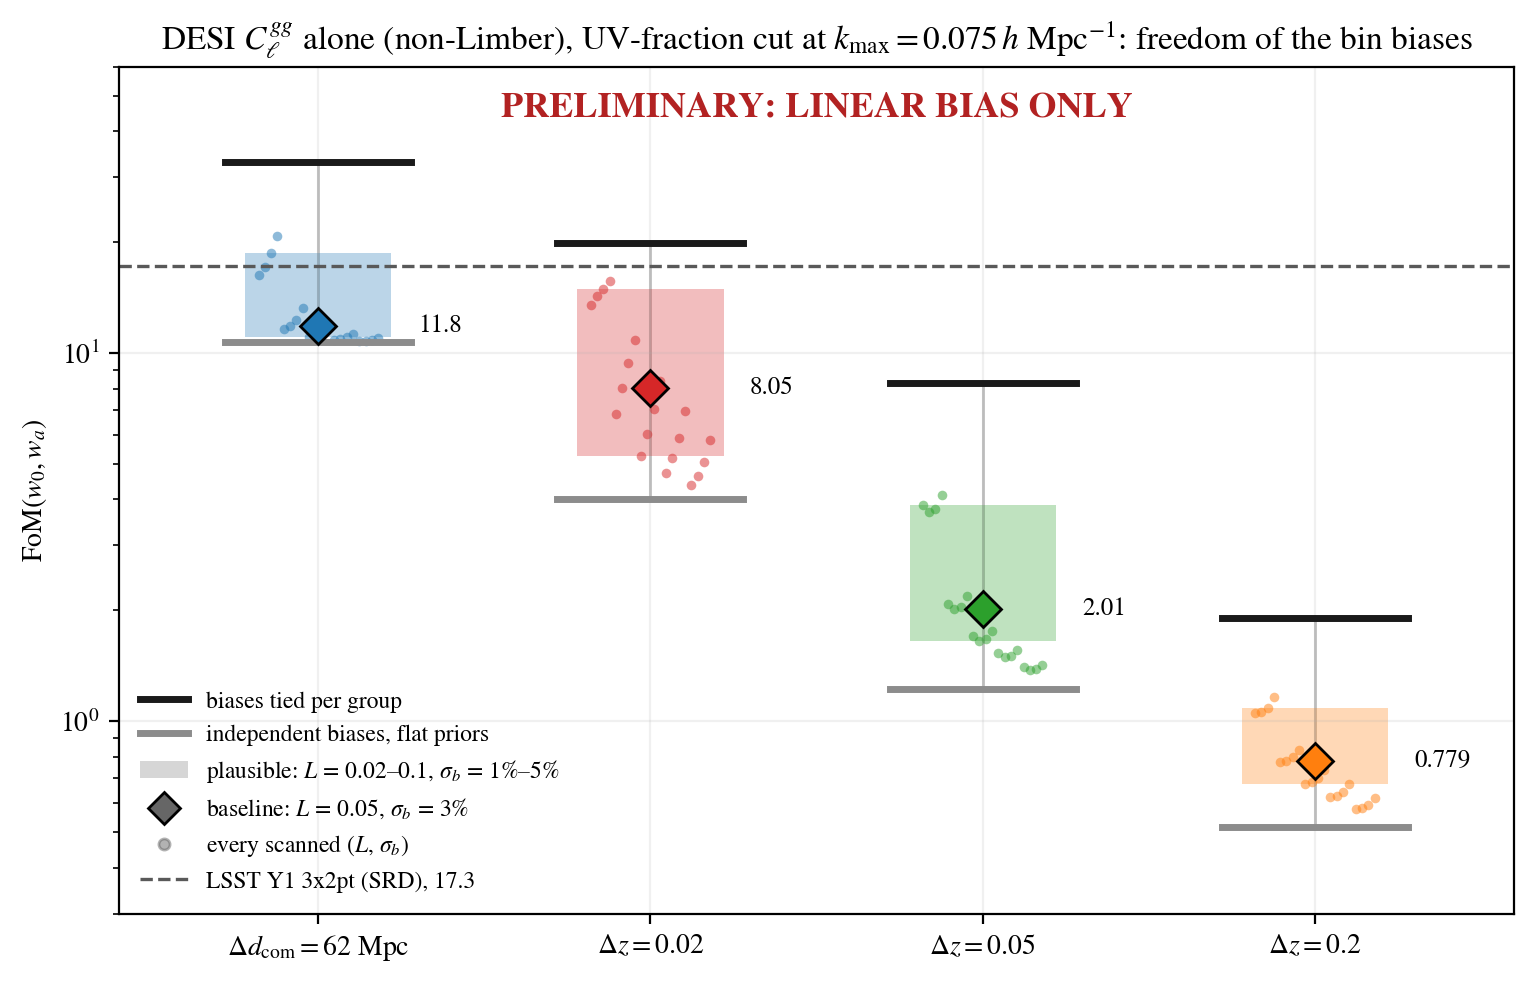
\includegraphics[width=\linewidth]{figures/fom_range.png}
  \caption{The ${\rm FoM}(w_0, w_a)$ of each thin-bin layout: the
    tied model (black cap), independent biases (gray cap), every
    scanned $(L, \sigma_b)$ point (dots), the plausible region
    ($\sigma_b = 1$--$5\%$, $L = 0.02$--$0.1$; band), the baseline
    (diamond), and the LSST Y1 3x2pt reference at $17.3$ (dashed).}
  \label{fig:range}
\end{figure}

Figure~\ref{fig:heatmap} resolves the same numbers on the
$(L, \sigma_b)$ grid.  $\Delta z = 0.02$ is the only layout where $L$
matters strongly: at $\sigma_b = 3\%$ its FoM runs from $6.8$ at
$L = 0.02$ to $10.9$ at $L = 0.2$.  The reason is the short neighbor
separation: with $\Delta z = 0.02$ the neighbor correlation
$e^{-\Delta z / L}$ stays high over the whole $L$ grid, from $0.37$
at $L = 0.02$ to $0.90$ at $L = 0.2$, so lengthening $L$ keeps
converting bin-to-bin freedom back into effective tying.  In the
other layouts the bins are as far apart as $L$ itself or farther, the
neighbor correlation is low everywhere on the grid, and $L$ moves the
FoM only weakly.

\begin{figure}[ht]
  \centering
  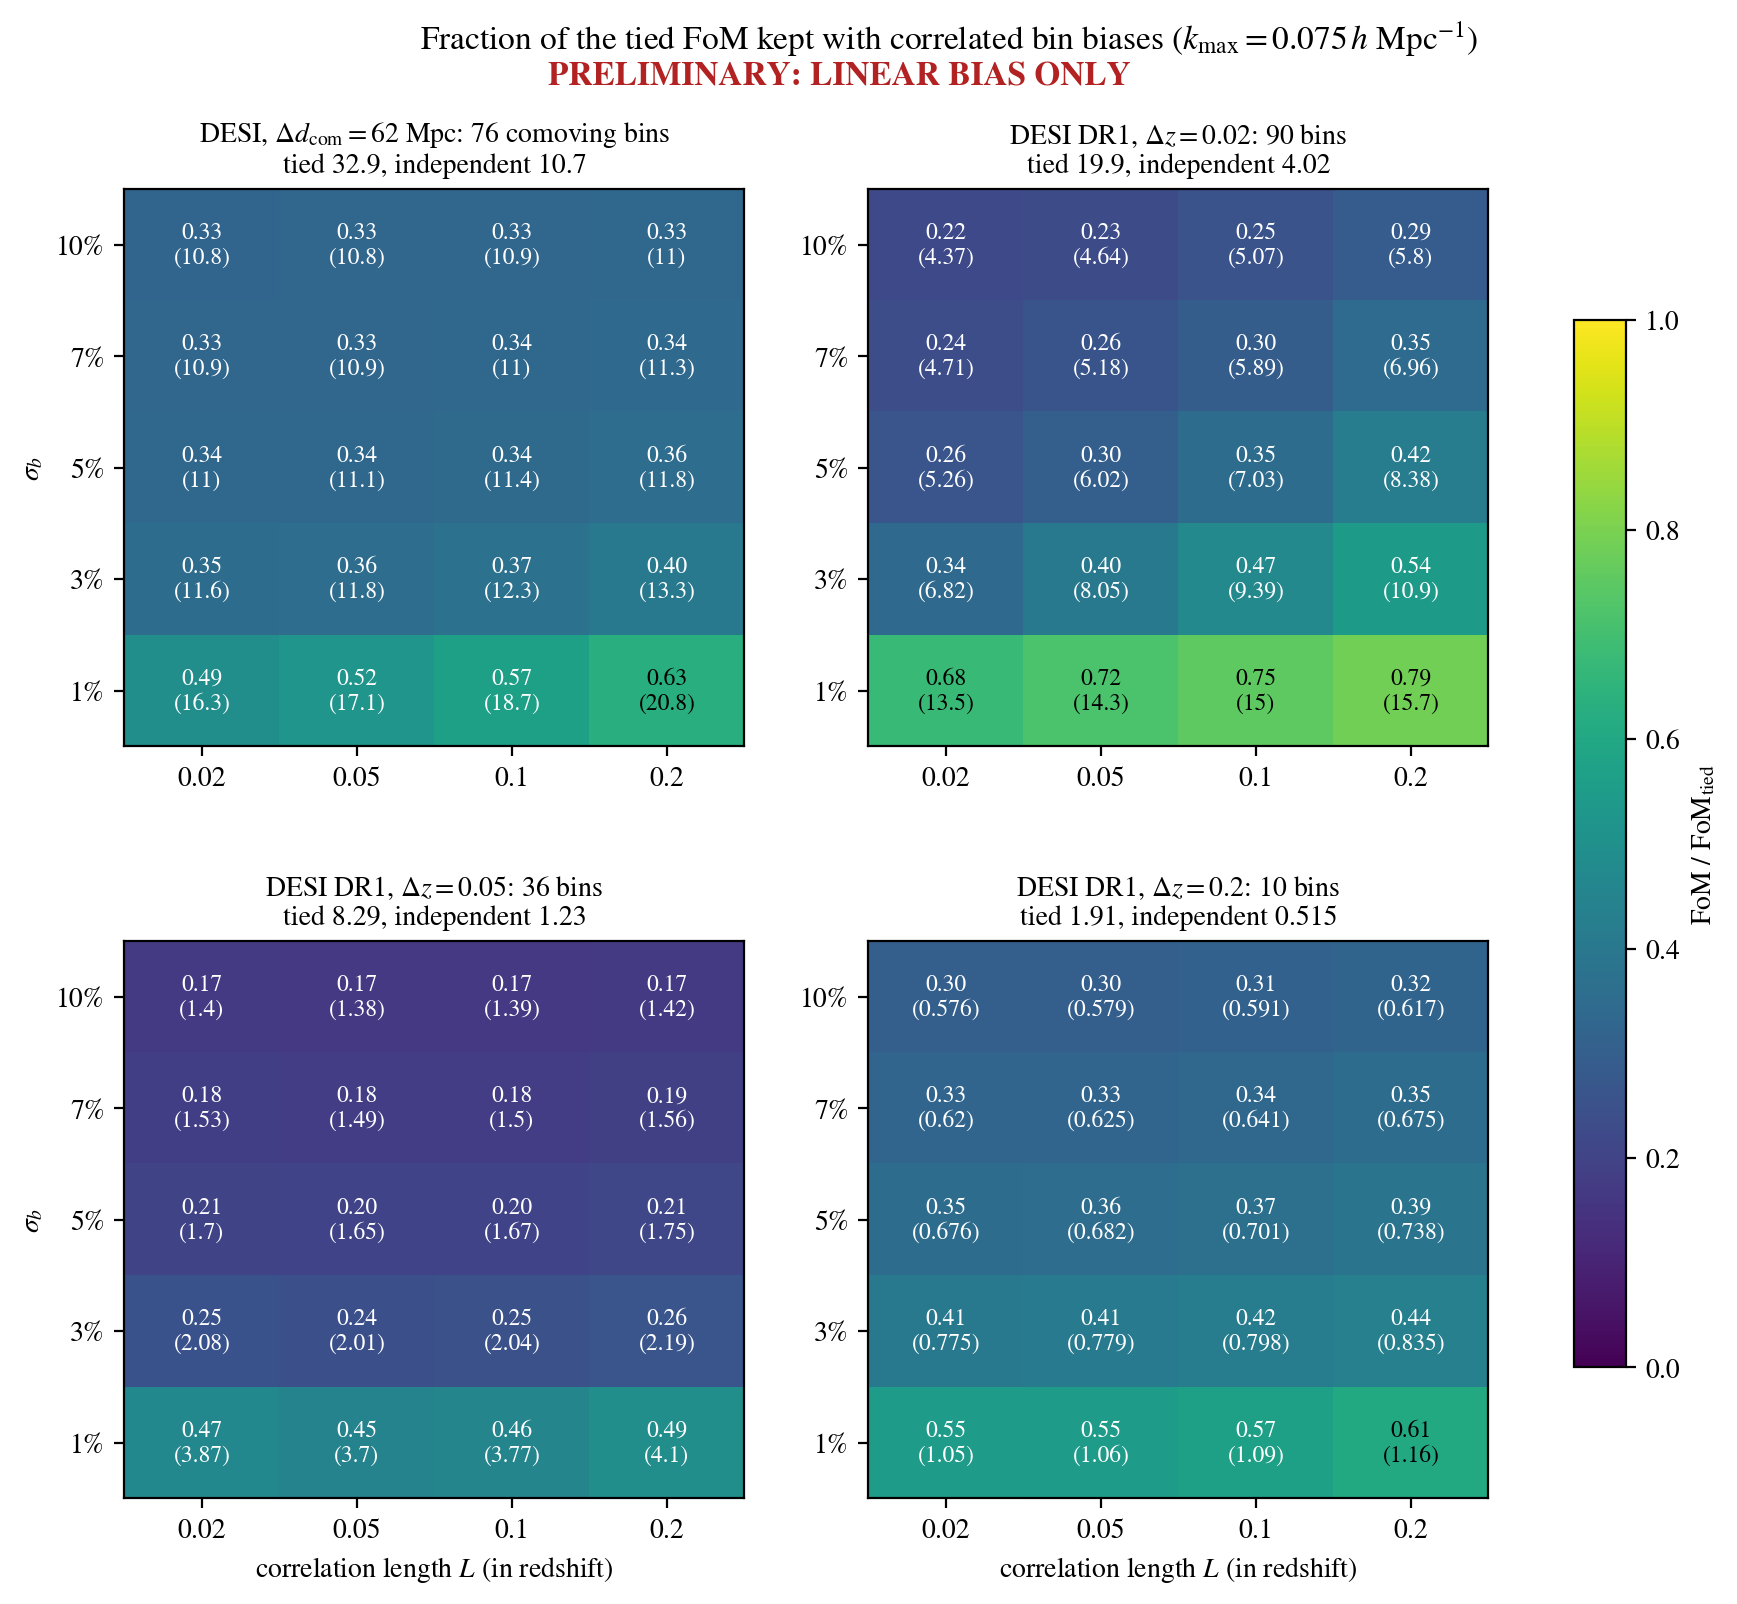
\includegraphics[width=\linewidth]{figures/fom_heatmap.png}
  \caption{${\rm FoM}/{\rm FoM}_{\rm tied}$ across the scanned
    $(L, \sigma_b)$ grid, one panel per layout, with the absolute FoM
    in parentheses.}
  \label{fig:heatmap}
\end{figure}

Figure~\ref{fig:collapse} tests whether one number controls the cost.
Its horizontal axis is $\sqrt{2}\,\kappa = \sigma_b \sqrt{2/L}$, the
rms neighbor change per unit $\sqrt{\Delta z}$ of
Eq.~\eqref{eq:roughness}.  The points do not collapse onto a single
curve per layout.  The reason is that the roughness controls only the
short-separation jumps: at fixed $\kappa$, a longer $L$ also carries
a larger wander $\sigma_b = \kappa \sqrt{L}$, so the bias can drift
coherently over the whole group, a freedom the roughness alone does
not capture.  The Fisher matrix pays for both kinds of freedom, so no
single-variable description of the grid should be expected.

\begin{figure}[ht]
  \centering
  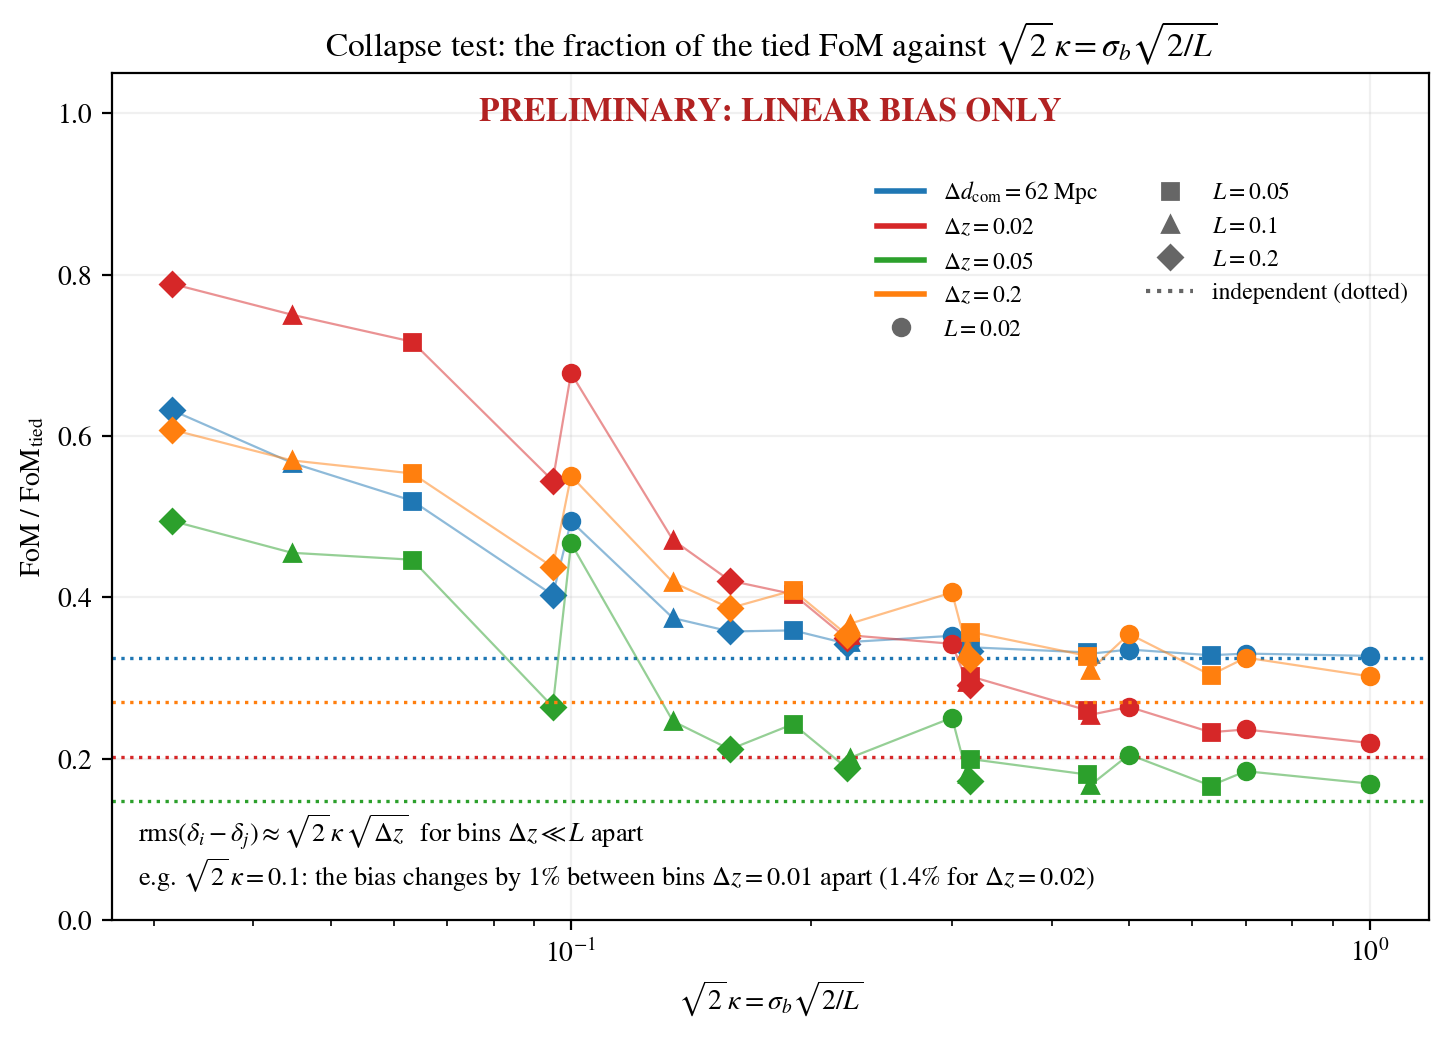
\includegraphics[width=\linewidth]{figures/fom_collapse.png}
  \caption{${\rm FoM}/{\rm FoM}_{\rm tied}$ against the roughness
    combination $\sqrt{2}\,\kappa = \sigma_b \sqrt{2/L}$.  Dotted
    lines: each layout's independent fraction
    ${\rm FoM}_{\rm indep}/{\rm FoM}_{\rm tied}$.  The points do not
    collapse onto a single curve per layout.}
  \label{fig:collapse}
\end{figure}

The scan reaches its two limits numerically, as Appendix~%
\ref{sec:limits} says it must.  At $\sigma_b = 0.01\%$ with
$L = 0.05$ the four layouts give ${\rm FoM} = 32.93$, $19.93$,
$8.285$ and $1.907$, against tied values $32.94$, $19.93$, $8.288$
and $1.908$; at $\sigma_b = 1000\%$ they land on the independent
values $10.69$, $4.016$, $1.225$ and $0.5154$ exactly.

\section*{Summary}
\label{sec:summary}

The intermediate bias model frees one amplitude $B_g$ per tracer group
and lets each bin deviate fractionally from the group's
constant-amplitude trend $B_g / D(z)$, with deviations correlated over a
redshift length $L$ and a per-bin wander $\sigma_b$.  In the Fisher
matrix this becomes one projected precision $\Prec$ per group, added to
the bin-amplitude block: $\Prec$ charges for differences between
neighboring amplitudes but never for a uniform shift of the group,
links only neighboring bins directly (the inverse covariance is
tridiagonal, even though the correlation itself reaches far), and
reduces to the tied model as
$L \to \infty$ and to independent flat-prior biases as
$\sigma_b \to \infty$.

\appendix

\section{The projected precision for two bins}
\label{sec:twobins}

Everything essential already happens with two bins.  Call their
amplitudes $\beta_1$ and $\beta_2$, with common fiducial value $B$,
prior spread $s$ per bin, and correlation coefficient $r$ between the
two deviations.  The prior covariance and its inverse are
\begin{equation}
  \Cov \;=\; s^2
  \begin{pmatrix} 1 & r \\ r & 1 \end{pmatrix},
  \qquad
  \Cov^{-1} \;=\; \frac{1}{s^2\,(1 - r^2)}
  \begin{pmatrix} 1 & -r \\ -r & 1 \end{pmatrix}.
  \label{eq:twobinC}
\end{equation}
(The inverse is checked by multiplying: the off-diagonal of
$\Cov\,\Cov^{-1}$ is $r - r = 0$ and the diagonal is
$(1 - r^2)/(1 - r^2) = 1$.)

Now examine the prior penalty
$\chi^2_{\rm prior} = \Delta\beta\T\, \Cov^{-1} \Delta\beta$, where
$\Delta\beta = (\beta_1 - B,\ \beta_2 - B)\T$ is the displacement from
the fiducial.  Two kinds of move matter.

\paragraph{A uniform shift.}
Take $\Delta\beta = a\,(1, 1)\T$: both bins move up by the same amount
$a$.  Working out the quadratic form with Eq.~\eqref{eq:twobinC},
\begin{equation}
  \Delta\beta\T \Cov^{-1} \Delta\beta
  \;=\;
  \frac{a^2}{s^2 (1 - r^2)}\,
  \bigl[\,(1 - r) + (1 - r)\,\bigr]
  \;=\;
  \frac{2 a^2}{s^2\,(1 + r)}
  \;\neq\; 0 .
  \label{eq:shiftpenalty}
\end{equation}
The plain prior charges for a uniform shift.  But a uniform shift of
all $\beta_i$ is a change of $B_g$, a direction the tied model leaves
completely free.  If the intermediate model kept this penalty, it would
constrain $B_g$ and the comparison between the models would be unfair.

\paragraph{A shape change.}
Take $\Delta\beta = a\,(1, -1)\T$: the bins move apart.  The same
algebra gives
\begin{equation}
  \Delta\beta\T \Cov^{-1} \Delta\beta
  \;=\;
  \frac{2 a^2}{s^2\,(1 - r)} .
  \label{eq:shapepenalty}
\end{equation}
This is the penalty the prior is \emph{meant} to apply: it grows
without bound as $r \to 1$, where the two bins are forced to track each
other, and it relaxes to the independent value $2a^2/s^2$ as
$r \to 0$.

A number makes the contrast concrete.  At $r = 0.670$ (the worked value
of Section~\ref{sec:jump}), the shape change costs
$2a^2/(0.330\,s^2) = 6.1\,a^2/s^2$ while the uniform shift costs
$2a^2/(1.670\,s^2) = 1.2\,a^2/s^2$.  The correlated prior already
charges five times more for the shape change than for the uniform
shift; the projection below takes the uniform-shift charge all the way
to zero.

\paragraph{The projected precision.}
The repair for the uniform shift is the projection $\Prec$ of
Eq.~\eqref{eq:projdef}.  Appendix~\ref{sec:threeviews} explains where
the formula comes from; here, compute it for two bins.
Because the two rows of $\Cov^{-1}$ have the
same sum, $\Cov^{-1}\ones = \bigl[s^2 (1+r)\bigr]^{-1} (1,1)\T$ and
$\ones\T \Cov^{-1} \ones = 2 / \bigl[s^2 (1+r)\bigr]$.  Substituting
into Eq.~\eqref{eq:projdef} and simplifying each entry,
\begin{equation}
  \Prec \;=\;
  \frac{1}{2 s^2 (1 - r)}
  \begin{pmatrix} 1 & -1 \\ -1 & 1 \end{pmatrix},
  \qquad
  \Delta\beta\T \Prec\, \Delta\beta
  \;=\;
  \frac{(\beta_1 - \beta_2)^2}{2 s^2 (1 - r)} .
  \label{eq:twobinP}
\end{equation}
The projected prior charges only for the \emph{difference} of the two
amplitudes.  A uniform shift, $\beta_1 = \beta_2$, is now free, as in
the tied model; a shape change keeps exactly the penalty of
Eq.~\eqref{eq:shapepenalty}.

The denominator is not an arbitrary constant.  With
$\mathrm{Var}(\beta_i) = s^2$ and
$\mathrm{Cov}(\beta_1, \beta_2) = s^2 r$,
\begin{equation}
  \mathrm{Var}(\beta_1 - \beta_2)
  \;=\; s^2 + s^2 - 2 s^2 r
  \;=\; 2 s^2 (1 - r):
  \label{eq:jumpvar2}
\end{equation}
the projected penalty is the squared jump between the bins divided by
the prior variance of that jump.  The whole construction reduces to one
sentence: \emph{the prior constrains the jump, not the level.}

\section{Why the projection ``sees'' the uniform shift: three views}
\label{sec:threeviews}

Equation~\eqref{eq:projdef} subtracts from $\Cov^{-1}$ a matrix built
out of the single vector $v = \Cov^{-1}\ones$: the subtracted piece is
$v\,v\T$ divided by the number $\ones\T \Cov^{-1} \ones$.  A matrix
built from one vector acts along one direction only, so the subtraction
removes the prior's information about exactly one direction, the
uniform shift, and leaves everything else alone.  This section
derives the formula three times, each derivation adding its own
intuition.  Throughout, a group has $n$ bins; $\Delta\beta$ and $\ones$
are vectors with $n$ entries.

\subsection{View (a): subtracting the best-fitting uniform shift}
\label{sec:viewa}

Ask the following question: given a displacement $\Delta\beta$, how much
of it can be explained as a pure change of the group amplitude?  A
change of $B_g$ by $c$ moves every $\beta_i$ by $c$, so the candidate
explanation is $c\,\ones$, and the unexplained part should be judged by
the prior metric.  Minimize over the scalar $c$ the quadratic form
\begin{equation}
  \chi^2(c)
  \;=\;
  \bigl(\Delta\beta - c\,\ones\bigr)\T
  \Cov^{-1}
  \bigl(\Delta\beta - c\,\ones\bigr).
  \label{eq:chi2c}
\end{equation}
Differentiating with respect to $c$ (the two cross terms are equal
because $\Cov^{-1}$ is symmetric),
\begin{equation}
  \frac{d\chi^2}{dc}
  \;=\;
  -2\,\ones\T \Cov^{-1} \bigl(\Delta\beta - c\,\ones\bigr)
  \;=\; 0,
  \qquad
  \frac{d^2\chi^2}{dc^2}
  \;=\;
  2\,\ones\T \Cov^{-1} \ones \;>\; 0,
  \label{eq:focs}
\end{equation}
where the second derivative is positive because $\Cov^{-1}$ is positive
definite, so the solution of the first equation is the minimum of
$\chi^2(c)$.  That solution is
\begin{equation}
  a \;=\;
  \frac{\ones\T \Cov^{-1} \Delta\beta}{\ones\T \Cov^{-1} \ones} .
  \label{eq:besta}
\end{equation}
For a diagonal $\Cov$ with variances $s_i^2$ this reduces to
$a = \sum_i \Delta\beta_i / s_i^2 \big/ \sum_i 1/s_i^2$, the familiar
inverse-variance weighted mean; Eq.~\eqref{eq:besta} is its
generalization to correlated errors: generalized least squares for a
constant.

Keep the dimensions straight: $\Delta\beta$, $\ones$ and the residual
$w = \Delta\beta - a\,\ones$ are vectors with $n$ entries; $a$ is a
single number.  The residuals $w$ satisfy one linear constraint
(Eq.~\eqref{eq:ortho} below), so they span $n - 1$ dimensions: one
direction of the $n$-dimensional displacement space has been handed to
the amplitude, and $n - 1$ directions of genuine shape freedom remain.

\subsection{View (b): a Pythagorean split of the penalty}
\label{sec:viewb}

Write the displacement as the best uniform shift plus a residual,
\begin{equation}
  \Delta\beta \;=\; a\,\ones + w .
  \label{eq:split}
\end{equation}
The first-order condition of Eq.~\eqref{eq:focs} says precisely that
\begin{equation}
  \ones\T \Cov^{-1} w \;=\; 0:
  \label{eq:ortho}
\end{equation}
the residual is orthogonal to the uniform direction \emph{in the
$\Cov^{-1}$ metric}.  (With correlated errors, "orthogonal" must be
measured with the same matrix that measures lengths.)  Substituting the
split into the full penalty, the cross term is
$2 a\,\ones\T \Cov^{-1} w = 0$, and
\begin{equation}
  \Delta\beta\T \Cov^{-1} \Delta\beta
  \;=\;
  a^2\, \ones\T \Cov^{-1} \ones
  \;+\;
  w\T \Cov^{-1} w .
  \label{eq:pythagoras}
\end{equation}
This is the Pythagorean theorem in the prior metric: the squared length
of the displacement is the squared length of its uniform piece plus the
squared length of its shape piece.

Now compare with the projection.  Inserting Eq.~\eqref{eq:besta} into
the subtracted term of Eq.~\eqref{eq:projdef} shows that the subtraction
removes exactly $a^2\,\ones\T \Cov^{-1} \ones$, the uniform piece.
What remains is
\begin{equation}
  \Delta\beta\T \Prec\, \Delta\beta
  \;=\;
  w\T \Cov^{-1} w .
  \label{eq:Pisw}
\end{equation}
Two consequences follow immediately.  First, a pure uniform shift has
$w = 0$, so its penalty vanishes.  Equivalently $\Prec\,\ones = 0$:
the projected matrix sends the uniform direction to zero and charges
nothing for it.  Second, a pure shape change (a displacement that
already satisfies Eq.~\eqref{eq:ortho}) has $a = 0$ and keeps its
original penalty untouched.  The projection removes one direction and
alters nothing else.

\subsection{View (c): marginalizing a flat-prior amplitude}
\label{sec:viewc}

The third view explains why the projection, rather than some other
uniform-shift repair, is the \emph{correct} prior.  Model the group
amplitudes as
\begin{equation}
  \beta \;=\; B\,\ones + \varepsilon,
  \qquad
  \varepsilon \sim \mathcal{N}(0, \Cov),
  \label{eq:genmodel}
\end{equation}
with a flat prior on the scalar $B$.  This is literally the
intermediate model of Eq.~\eqref{eq:model}, linearized around the
fiducial.  The prior density of $\beta$ is obtained by integrating $B$
out:
\begin{equation}
  p(\beta) \;\propto\;
  \int dB\,
  \exp\!\left[
    -\tfrac{1}{2}
    \bigl(\beta - B\,\ones\bigr)\T \Cov^{-1} \bigl(\beta - B\,\ones\bigr)
  \right].
  \label{eq:marg}
\end{equation}
The exponent is quadratic in $B$.  Writing
$S = \ones\T \Cov^{-1} \ones$ and completing the square,
\begin{equation}
  \bigl(\beta - B\ones\bigr)\T \Cov^{-1} \bigl(\beta - B\ones\bigr)
  \;=\;
  S\,\bigl(B - B_*\bigr)^2
  \;+\;
  \beta\T \Cov^{-1} \beta
  \;-\;
  \frac{\bigl(\ones\T \Cov^{-1} \beta\bigr)^2}{S},
  \qquad
  B_* = \frac{\ones\T \Cov^{-1} \beta}{S} .
  \label{eq:complsq}
\end{equation}
The $B$ integral is a Gaussian centered on $B_*$ with width
$1/\sqrt{S}$; it contributes only a $\beta$-independent constant
$\sqrt{2\pi / S}$.  What survives in the exponent is
\begin{equation}
  p(\beta) \;\propto\;
  \exp\!\left[-\tfrac{1}{2}\, \beta\T \Prec\, \beta\right],
  \qquad
  \Prec \;=\; \Cov^{-1}
  - \frac{\Cov^{-1}\ones\,\ones\T \Cov^{-1}}{\ones\T \Cov^{-1} \ones},
  \label{eq:margresult}
\end{equation}
exactly the projection of Eq.~\eqref{eq:projdef}.

The same computation has a standard matrix name.  Expanding the
exponent of Eq.~\eqref{eq:marg} in the joint variables $(\beta, B)$
gives a Gaussian with the $(n+1) \times (n+1)$ block precision
\begin{equation}
  \mathsf{F}_{(\beta, B)}
  \;=\;
  \begin{pmatrix}
    \Cov^{-1} & -\,\Cov^{-1}\ones \\[0.4ex]
    -\,\ones\T \Cov^{-1} & \ones\T \Cov^{-1} \ones
  \end{pmatrix}.
  \label{eq:jointprec}
\end{equation}
Removing a parameter from a precision matrix is not just deleting its
row and column: the remaining block must also be corrected downward by
whatever the removed parameter could absorb.  The corrected block,
$\Prec = \mathsf{F}_{\beta\beta}
- \mathsf{F}_{\beta B}\, \mathsf{F}_{BB}^{-1}\, \mathsf{F}_{B\beta}$,
is called the \emph{Schur complement} over $B$, and it reproduces
Eq.~\eqref{eq:projdef} term by term.  So $\Prec$ is not a trick: it
is precisely the statement "\emph{$B_g$ is sampled with a flat prior
and marginalized}", folded into one matrix.

Note also that $B_*$ in Eq.~\eqref{eq:complsq} is the same
generalized-least-squares mean as $a$ in Eq.~\eqref{eq:besta}: the
marginalization integrates over all amplitudes, and the best-fitting
one dominates the integral.

\subsection{Checking views (b) and (c) on the two-bin case}
\label{sec:check2}

For $n = 2$ the rows of $\Cov^{-1}$ in Eq.~\eqref{eq:twobinC} have
equal sums, so Eq.~\eqref{eq:besta} gives the plain mean,
$a = (\Delta\beta_1 + \Delta\beta_2)/2$, and the residual is the
antisymmetric half-difference,
$w = \tfrac{1}{2}(\Delta\beta_1 - \Delta\beta_2)\,(1, -1)\T$.  Its
penalty, using the shape-change result of Eq.~\eqref{eq:shapepenalty}
with $a \to \tfrac{1}{2}(\Delta\beta_1 - \Delta\beta_2)$, is
\begin{equation}
  w\T \Cov^{-1} w
  \;=\;
  \frac{2}{s^2 (1-r)}
  \left(\frac{\Delta\beta_1 - \Delta\beta_2}{2}\right)^{\!2}
  \;=\;
  \frac{(\Delta\beta_1 - \Delta\beta_2)^2}{2 s^2 (1 - r)},
  \label{eq:check2}
\end{equation}
which is the direct two-bin computation of Eq.~\eqref{eq:twobinP}.
Views (a), (b) and (c) all land on the same matrix.

\section{Many bins and several groups}
\label{sec:general}

\subsection{Three bins: total correlation versus direct links}
\label{sec:kernel}

A group now has $n$ bins at redshifts $z_1 < z_2 < \dots < z_n$,
unevenly spaced in general, with the prior covariance of
Eq.~\eqref{eq:covdef},
\begin{equation}
  \Cov_{ij} \;=\; s^2 \exp\!\left(-\,\frac{|z_i - z_j|}{L}\right).
  \label{eq:nbinC}
\end{equation}
This matrix is positive definite for any set of distinct redshifts
(all its eigenvalues are positive), so the prior is a proper
probability distribution and $\Cov^{-1}$ exists.

The structure of $\Cov^{-1}$ is best seen on three evenly spaced bins.
With neighbor correlation $r = e^{-\Delta z / L}$, the outer pair sits
two steps apart and carries $e^{-2\Delta z / L} = r^2$, so
\begin{equation}
  \Cov \;=\; s^2
  \begin{pmatrix} 1 & r & r^2 \\ r & 1 & r \\ r^2 & r & 1 \end{pmatrix},
  \qquad
  \Cov^{-1} \;=\; \frac{1}{s^2\,(1 - r^2)}
  \begin{pmatrix} 1 & -r & 0 \\ -r & 1 + r^2 & -r \\ 0 & -r & 1
  \end{pmatrix}.
  \label{eq:threebin}
\end{equation}
One multiplication confirms the surprising entry.  The $(1,3)$ entry of
$\Cov^{-1}\Cov$ must be zero (it is an off-diagonal entry of the
identity matrix), and indeed row 1 of $\Cov^{-1}$ times column 3 of
$\Cov$ gives, dropping the prefactors,
\begin{equation}
  1 \cdot r^2 \;+\; (-r) \cdot r \;+\; 0 \cdot 1
  \;=\; r^2 - r^2 \;=\; 0 .
  \label{eq:rowcheck}
\end{equation}

Here is the point that looks paradoxical at first.  Bins 1 and 3
\emph{are} correlated ($\Cov$ contains $r^2$), yet their entry in
$\Cov^{-1}$ is exactly zero.  The two matrices answer different
questions.  $\Cov$ gives the \emph{total} correlation: what $\delta_1$
tells you about $\delta_3$ when nothing else is known.  $\Cov^{-1}$
gives the \emph{direct} correlation: what $\delta_1$ still tells you
about $\delta_3$ once $\delta_2$ is already known, and that is
nothing.  All of the 1--3 correlation travels through bin 2.

Think of a chain of people passing a message.  The first person's
message reaches far down the chain, but the links are only between
neighbors: nobody talks past the person standing next to them.

The exponential kernel is special in making this exact, because its
correlations multiply along the chain:
\begin{equation}
  e^{-(z_3 - z_1)/L}
  \;=\;
  e^{-(z_3 - z_2)/L}\; e^{-(z_2 - z_1)/L} .
  \label{eq:factorize}
\end{equation}
The long-distance correlation is the product of the step correlations,
so the middle bin already carries everything the outer bins share.  A
Gaussian kernel $e^{-\Delta z^2 / L^2}$ does not factorize this way,
because the squared separations do not add up along the chain:
$(z_3 - z_1)^2 \neq (z_3 - z_2)^2 + (z_2 - z_1)^2$.  Its inverse
is dense.

The same structure shows directly in the penalty.  For $n$ evenly
spaced bins, the quadratic form of the deviations $\delta_i$ (whose
covariance is $\sigma_b^2 \mathsf{R}$) regroups into a sum over
neighbor links,
\begin{equation}
  \delta\T \bigl(\sigma_b^2 \mathsf{R}\bigr)^{-1} \delta
  \;=\;
  \frac{\delta_1^2}{\sigma_b^2}
  \;+\;
  \sum_{k=1}^{n-1}
  \frac{\bigl(\delta_{k+1} - r\,\delta_k\bigr)^2}
       {\sigma_b^2\,(1 - r^2)} .
  \label{eq:chainsum}
\end{equation}
Each term compares one bin with $r$ times the bin before it: every bin
is pulled only by its neighbor, and the long-range correlation comes
from chaining the pulls.  (Expanding the squares and collecting terms
reproduces Eq.~\eqref{eq:threebin} for $n = 3$; Appendix~\ref{app:chain}
does it for general, uneven spacing.)  This is the precise sense of
"correlation only between adjacent bins": \emph{directly}, only
neighbors talk; \emph{in total}, the influence propagates down the
whole chain.  Probability theory calls this neighbors-only structure
the Markov property.

\subsection{The tridiagonal inverse for $n$ bins}
\label{sec:tridiag}

A matrix whose nonzero entries sit only on the diagonal and the two
neighboring off-diagonals is called \emph{tridiagonal}.  The three-bin
inverse of Eq.~\eqref{eq:threebin} is the smallest interesting example,
and the pattern grows unchanged.  For $n$ evenly spaced bins, where
every adjacent pair has the same correlation $r = e^{-\Delta z / L}$
and $\Cov_{ij} = s^2\, r^{|i - j|}$,
\begin{equation}
  \Cov^{-1} \;=\;
  \frac{1}{s^2\,(1 - r^2)}
  \begin{pmatrix}
    1      & -r     &        &        &        \\
    -r     & 1+r^2  & -r     &        &        \\
           & -r     & \ddots & \ddots &        \\
           &        & \ddots & 1+r^2  & -r     \\
           &        &        & -r     & 1
  \end{pmatrix},
  \label{eq:ar1}
\end{equation}
with diagonal $(1,\ 1+r^2,\ \dots,\ 1+r^2,\ 1)$, off-diagonal entries
$-r$, blanks zero, and the overall factor $1/\bigl[s^2(1-r^2)\bigr]$.
The entries read off the chain sum of Eq.~\eqref{eq:chainsum}.  An
off-diagonal entry is the link between that pair of neighbors.  An
interior bin touches two links, one to the bin on its left and one to
the bin on its right, and the two pulls together contribute
$1 + r^2$; the first and last bins touch only one link each, hence the
plain $1$ in the corners.

With uneven spacing, each adjacent pair has its own step and therefore
its own correlation,
\begin{equation}
  r_k \;=\; \exp\!\left(-\,\frac{z_{k+1} - z_k}{L}\right),
  \qquad k = 1, \dots, n-1 ,
  \label{eq:rk}
\end{equation}
and the inverse keeps the same shape with per-pair entries:
\begin{equation}
  s^2\,\bigl(\Cov^{-1}\bigr)_{kk} =
  \begin{cases}
    \dfrac{1}{1 - r_1^2}, & k = 1,\\[2.2ex]
    \dfrac{1}{1 - r_{k-1}^2} + \dfrac{r_k^2}{1 - r_k^2}, & 1 < k < n,\\[2.2ex]
    \dfrac{1}{1 - r_{n-1}^2}, & k = n,
  \end{cases}
  \qquad
  s^2\,\bigl(\Cov^{-1}\bigr)_{k, k+1} = \frac{-\,r_k}{1 - r_k^2}.
  \label{eq:uneven}
\end{equation}
In words: the off-diagonal entry is the neighbor link of pair $k$,
stronger when the bins are closer ($r_k$ nearer one); the diagonal
entry of bin $k$ collects the links touching that bin, one term from
the pair on its left and one from the pair on its right; the first and
last bins carry one link only.  Setting all $r_k = r$ turns the
interior diagonal into
$1/(1-r^2) + r^2/(1-r^2) = (1+r^2)/(1-r^2)$ and recovers
Eq.~\eqref{eq:ar1}.  Appendix~\ref{app:chain} derives
Eq.~\eqref{eq:uneven} from the chain of neighbor links; the companion
script \texttt{verify\_prior.py} checks the three-bin, even and uneven
forms numerically.

\subsection{The projection, group by group}
\label{sec:projgroups}

Each group receives the projected precision of Eq.~\eqref{eq:projdef},
built from its own $\Cov$.  The properties derived in
Appendix~\ref{sec:threeviews} carry over verbatim to $n$ bins.
$\Prec\,\ones = 0$: a uniform shift of the whole group costs nothing.
$\Prec$ is positive semidefinite, which means no displacement is
\emph{rewarded}: every move either costs $\chi^2$ or is free.  And of
the $n$ directions a group can move in, exactly one (the uniform shift)
is free while the other $n - 1$ are charged: in matrix language,
$\Prec$ has rank $n - 1$.

Several groups combine trivially.  The prior of
Eq.~\eqref{eq:priorkernel} is zero across groups, so the full prior
covariance is block-diagonal, one block per group; and each group has
its own free amplitude $B_g$, so each block is projected separately.
The total prior precision is the block-diagonal matrix of the per-group
projections.

\subsection{The two limits}
\label{sec:limits}

The intermediate model contains both extremes.

As $L \to \infty$, every $r_k \to 1$, so the jump variance
$2\sigma_b^2(1 - r_k)$ of every adjacent pair goes to zero: the prior
forces all deviations of a group to be equal.  The only freedom left is
their common value, a uniform shift, and that is the direction the
projection leaves free.  This is the tied model, with one free $B_g$
per group, \emph{whatever} the value of $\sigma_b$.

As $\sigma_b \to \infty$ at fixed $L$, the overall scale of $\Cov$
diverges, so $\Cov^{-1} \to 0$ and with it $\Prec \to 0$: the prior
penalty vanishes and every bin's amplitude is free: the independent
model with flat priors.

Between the limits, $L$ and $\sigma_b$ interpolate continuously, which
is what makes the model useful: the figure of merit can be traced as a
function of how much bin-to-bin freedom the bias is granted.

\section{The tridiagonal inverse from the chain of links}
\label{app:chain}

Because correlations multiply along the chain
(Eq.~\eqref{eq:factorize}), the prior can be built one bin at a time:
the joint density of the deviations factorizes into neighbor
conditionals,
\begin{equation}
  p(\delta_1, \dots, \delta_n)
  \;=\;
  p(\delta_1)\, p(\delta_2 \mid \delta_1) \cdots
  p(\delta_n \mid \delta_{n-1}),
  \label{eq:chainfactor}
\end{equation}
where each conditional is Gaussian with
\begin{equation}
  \bigl\langle \delta_{k+1} \mid \delta_k \bigr\rangle
  \;=\; r_k\,\delta_k,
  \qquad
  \mathrm{Var}\bigl(\delta_{k+1} \mid \delta_k\bigr)
  \;=\; \sigma_b^2\,\bigl(1 - r_k^2\bigr).
  \label{eq:conditional}
\end{equation}
Here $r_k = e^{-(z_{k+1} - z_k)/L}$ is, as in
Sections~\ref{sec:jump} and \ref{sec:tridiag}, the correlation
coefficient of the adjacent bins $k$ and $k+1$: the kernel of
Eq.~\eqref{eq:priorkernel} gives
$\mathrm{Cov}(\delta_k, \delta_{k+1}) = \sigma_b^2\, r_k$ and
$\mathrm{Var}(\delta_k) = \mathrm{Var}(\delta_{k+1}) = \sigma_b^2$.

The conditional mean and variance in Eq.~\eqref{eq:conditional} follow
from nothing more than these covariances.  Split $\delta_{k+1}$ into
the part predicted by its neighbor and a leftover $e$,
\begin{equation}
  \delta_{k+1} \;=\; a\,\delta_k + e ,
  \label{eq:splitleftover}
\end{equation}
and choose the number $a$ so that the leftover carries no correlation
with $\delta_k$:
\begin{equation}
  \mathrm{Cov}(e, \delta_k)
  \;=\;
  \mathrm{Cov}(\delta_{k+1}, \delta_k) - a\,\mathrm{Var}(\delta_k)
  \;=\;
  \sigma_b^2\, r_k - a\,\sigma_b^2
  \;=\; 0
  \quad\Longrightarrow\quad
  a = r_k .
  \label{eq:leftovera}
\end{equation}
The leftover's variance follows by expanding
$e = \delta_{k+1} - r_k \delta_k$:
\begin{equation}
  \mathrm{Var}(e)
  \;=\;
  \mathrm{Var}(\delta_{k+1})
  - 2 r_k\, \mathrm{Cov}(\delta_{k+1}, \delta_k)
  + r_k^2\, \mathrm{Var}(\delta_k)
  \;=\;
  \sigma_b^2 - 2 r_k^2 \sigma_b^2 + r_k^2 \sigma_b^2
  \;=\;
  \sigma_b^2\,\bigl(1 - r_k^2\bigr).
  \label{eq:leftovervar}
\end{equation}
For jointly Gaussian variables, uncorrelated means independent.  So
once $\delta_k$ is known, the only randomness left in
$\delta_{k+1} = r_k \delta_k + e$ is $e$ itself: the conditional mean
is $r_k \delta_k$ and the conditional variance is
$\sigma_b^2 (1 - r_k^2)$, which is Eq.~\eqref{eq:conditional}.  In one
line: knowing the neighbor explains the fraction $r_k^2$ of the bin's
variance, and the fraction $1 - r_k^2$ is new.

The factorization of Eq.~\eqref{eq:chainfactor} needs one more fact:
conditioning on $\delta_k$ alone must be enough: the earlier bins
must add nothing.  This is again the multiplication of correlations
along the chain.  For any earlier bin $j \le k$,
\begin{equation}
  \mathrm{Cov}(e, \delta_j)
  \;=\;
  \sigma_b^2
  \left[
    e^{-(z_{k+1} - z_j)/L} - r_k\, e^{-(z_k - z_j)/L}
  \right]
  \;=\;
  \sigma_b^2\, e^{-(z_k - z_j)/L}
  \left[
    e^{-(z_{k+1} - z_k)/L} - r_k
  \right]
  \;=\; 0 ,
  \label{eq:pastfree}
\end{equation}
because the first exponential factorizes through $z_k$ and the bracket
is $r_k - r_k$.  The leftover is therefore independent of every earlier
bin, and the chain of one-step conditionals is the complete prior.

Taking $-2 \ln p$ of Eq.~\eqref{eq:chainfactor} gives the penalty as
the chain sum, the uneven-spacing version of
Eq.~\eqref{eq:chainsum}:
\begin{equation}
  \delta\T \bigl(\sigma_b^2 \mathsf{R}\bigr)^{-1} \delta
  \;=\;
  \frac{\delta_1^2}{\sigma_b^2}
  \;+\;
  \sum_{k=1}^{n-1}
  \frac{\bigl(\delta_{k+1} - r_k\,\delta_k\bigr)^2}
       {\sigma_b^2\,\bigl(1 - r_k^2\bigr)} .
  \label{eq:chainsumuneven}
\end{equation}
Expanding each square and collecting the coefficient of every product
$\delta_i \delta_j$ reads off the precision matrix entry by entry.
$\delta_1^2$ appears twice: in the first term (coefficient $1$) and in
the $k = 1$ link as the predictor (coefficient $r_1^2/(1 - r_1^2)$);
the two add up to $1/(1 - r_1^2)$.  An interior $\delta_k^2$ appears in
the $k-1$ link as the predicted bin ($1/(1 - r_{k-1}^2)$) and in the
$k$ link as the predictor ($r_k^2/(1 - r_k^2)$).  The last bin is only
ever predicted: $1/(1 - r_{n-1}^2)$.  Each product
$\delta_k \delta_{k+1}$ appears in its own link only, with coefficient
$-2 r_k/(1 - r_k^2)$, i.e.\ a symmetric matrix entry
$-r_k/(1 - r_k^2)$.  No product of non-neighbors ever appears, so the
matrix is tridiagonal by construction.  This is Eq.~\eqref{eq:uneven}
in units of $\sigma_b^2$; replacing $\delta$ by
$\Delta\beta = B_g\,\delta$ and $\sigma_b$ by $s = \sigma_b B_g$ gives
the same matrix for the bin amplitudes.

\section{The bias continuity equation, step by step}
\label{app:continuity}

The matter density $\rho_m(\mathbf{x}, t)$ defines the matter
overdensity $\delta_m = (\rho_m - \bar\rho_m)/\bar\rho_m$, with
$\bar\rho_m(t)$ the mean density; the galaxy number density $n_g$
defines the galaxy-count overdensity $\delta_g$ the same way.
Conservation of mass and of galaxy number gives each field a
continuity equation.  In comoving coordinates, keeping only terms
linear in the fluctuations (the product $\delta\,\mathbf{v}$ is
second order and dropped),
\begin{equation}
  \frac{d \delta_m}{dt}
  \;=\;
  -\,\frac{1}{a}\,\nabla \cdot \mathbf{v}_m,
  \qquad
  \frac{d \delta_g}{dt}
  \;=\;
  -\,\frac{1}{a}\,\nabla \cdot \mathbf{v}_g,
  \label{eq:continuity}
\end{equation}
where $t$ is cosmic time, $a$ the scale factor, and $\mathbf{v}_m$
and $\mathbf{v}_g$ the peculiar velocity fields of the matter and of
the galaxies.

The two velocity fields are the same.  On large scales the galaxies
carry no pressure of their own and fall in the same gravitational
potential as the matter, so a conserved sample rides the matter flow:
$\mathbf{v}_g = \mathbf{v}_m$.  This is the no-velocity-bias
assumption; Tegmark and Peebles \cite{TegmarkPeebles1998} state it as
galaxies behaving as test particles that fairly trace the large-scale
velocity field.

With equal right-hand sides, subtracting the two equations of
Eq.~\eqref{eq:continuity} leaves
\begin{equation}
  \frac{d}{dt}\bigl(\delta_g - \delta_m\bigr) \;=\; 0
  \quad\Longrightarrow\quad
  \delta_g(z) - \delta_m(z)
  \;=\;
  \delta_g(z_c) - \delta_m(z_c)
  \label{eq:frozen}
\end{equation}
after integrating in time from the reference redshift $z_c$ to any
other redshift $z$: the excess clumping keeps its initial value
forever.

Now substitute the bias.  At $z_c$ the sample has linear bias $b_c$,
so $\delta_g(z_c) = b_c\,\delta_m(z_c)$ and the frozen difference is
$(b_c - 1)\,\delta_m(z_c)$.  The matter grows as
$\delta_m(z) = \delta_m(z_c)\, D(z)/D(z_c)$, with $D$ the linear
growth factor.  Then
\begin{equation}
  \delta_g(z)
  \;=\;
  \delta_m(z) + \bigl(b_c - 1\bigr)\,\delta_m(z_c)
  \;=\;
  \delta_m(z)
  \left[\,1 + \bigl(b_c - 1\bigr)\,\frac{D(z_c)}{D(z)}\,\right],
  \label{eq:appsub}
\end{equation}
and dividing by $\delta_m(z)$ gives the bias
$b(z) = \delta_g/\delta_m$ of Eq.~\eqref{eq:fry}.  Dividing instead
by the tied bias $b_c\,D(z_c)/D(z)$ gives the deviation of
Eq.~\eqref{eq:tilt}, $\delta(z) = (D(z)/D(z_c) - 1)/b_c$: positive at
redshifts below $z_c$, where the matter has grown past its reference
value, and negative above.

The debiasing limit follows from Eq.~\eqref{eq:fry} alone.  As $D$
grows, the frozen term is divided by an ever larger number, so
$b \to 1$: from above when $b_c > 1$ and from below when $b_c < 1$.
Gravity debiases a conserved sample, because the part of $\delta_g$
that traces the matter keeps growing while the frozen excess does
not.

Tegmark and Peebles drop the assumption that $\delta_g$ is
proportional to $\delta_m$ point by point.  They describe the pair of
fields by three numbers: the matter fluctuation amplitude $\sigma$,
the bias $b$ (the ratio of the galaxy to the matter fluctuation
amplitude) and the correlation coefficient $r$ between the two
fields; $r < 1$ is stochastic bias, galaxies tracing the matter
imperfectly.  The same continuity argument evolves all three (their
section ``After the galaxy formation epoch''): with $D$ normalized to
one today and the subscript zero marking today,
\begin{equation}
  b_0 =
  \left[(1 - D)^2 + 2 D (1 - D)\, b\, r + D^2 b^2\right]^{1/2},
  \qquad
  r_0 = \frac{(1 - D) + D\, b\, r}{b_0},
  \label{eq:tpevol}
\end{equation}
where $b$ and $r$ are the values at the epoch whose growth factor is
$D$.

Both $b_0$ and $r_0$ approach one as clustering grows, whatever
their initial values: the matter-sourced part of the galaxy field
grows with $D$ while the frozen part does not, so the field is
progressively dominated by the piece that traces the matter.
Perfect correlation is a fixed point: for $r = 1$,
Eq.~\eqref{eq:tpevol} collapses to $b_0 - 1 = (b - 1)\,D$, which is
Eq.~\eqref{eq:fry} again.  The conserved population of this note is
the perfectly correlated special case of their model.

Each assumption fails in a specific way for a DESI sample.
Membership is not conserved: the flux limit and color cuts admit and
remove galaxies as redshift grows (the threshold drift and
color-selection features of Section~\ref{sec:selection}), mergers
turn two members into one, and an ELG belongs to the sample only
during its star-forming phase.  The no-velocity-bias and
linear-theory assumptions hold well on the scales this forecast
keeps; conservation is the assumption that breaks.

The script of Appendix~\ref{app:verify} integrates
Eq.~\eqref{eq:continuity} numerically, with $\delta_m$ from the
linear growth equation, and recovers the closed form of
Eq.~\eqref{eq:fry} to a relative accuracy of $2 \times 10^{-9}$.

\section{What the literature says, paper by paper}
\label{app:literature}

This appendix summarizes each measurement behind
Section~\ref{sec:evidence}, for a reader who has not read the papers.
The tags are those of that section: measured, derived, assumed.

\subsection{Passive-evolution tests of massive red galaxies}

\paragraph{Wake et al. \cite{Wake2008}.}
What was measured: the two-point correlation function of over
$10{,}000$ luminous red galaxies (LRGs) from SDSS and the 2SLAQ
survey at $0.19 < z < 0.55$, matched in rest-frame color and
luminosity, with stellar masses above $10^{11}\,h^{-1} M_\odot$.
Method: the redshift-space and real-space autocorrelation of the
matched samples, interpreted with a halo model.  Result: no
significant evolution of the correlation amplitude, but a strictly
merger-free passive model is rejected; a merger rate of
$7.5 \pm 2.3\%$ between $z = 0.55$ and $z = 0.19$, about $2.4\%$ per
Gyr, fits the data.  Implication here: LRG deviations from conserved
evolution are a few percent in number per Gyr (measured), and the
induced bias change is smaller, because merging moves galaxies
between halos of similar mass.

\paragraph{Tojeiro et al. \cite{Tojeiro2012}.}
What was measured: the merger rate and clustering evolution of
$250{,}000$ BOSS galaxies up to $z \approx 0.7$, connected to the
SDSS-I/II LRGs at lower redshift.  Method: each BOSS galaxy receives
a likelihood of being a progenitor of the LRG sample, built from the
fossil record of the LRGs (star-formation and metallicity
histories); the weighted sample's large-scale clustering is compared
between the surveys.  Result: the sample evolves by merging at
$2 \pm 1.5\%$ per Gyr, and the weighted clustering evolution is
consistent with dynamical passive evolution, the continuity-equation
prediction.  Implication here: the conserved shape holds to the
percent-per-Gyr level for these galaxies (measured).

\paragraph{Guo et al. \cite{Guo2013}.}
What was measured: the projected two-point correlation function of
about $260{,}000$ CMASS galaxies at $0.43 < z < 0.7$ (BOSS DR9).
Method: subsamples of fixed comoving number density built with
redshift-dependent magnitude thresholds, so that the same population
is followed across redshift.  Result: the clustering of the
fixed-density samples is consistent with passive evolution, and
red-sequence clustering at fixed luminosity shows no significant
evolution.  Implication here: the same (measured).

\subsection{The DESI luminous red galaxies}

\paragraph{Zhou et al. \cite{Zhou2021}.}
What was measured: the redshift-dependent clustering of 2.7 million
DESI-like LRGs over $5655$ square degrees at $0.4 < z < 0.9$, in
photometric-redshift bins of width $\Delta z \approx 0.1$.  Method:
projected correlation functions with photometric redshifts of
$0.02$ precision, fit with a five-parameter halo occupation
distribution (HOD).  Result: the HOD parameters show little
evolution except in the highest bin, and the bias follows a constant
clustering amplitude; Table~\ref{tab:zhou} lists the measured biases
and their residuals around $b = 1.5/D$ (derived here): within
$\pm 2.3\%$ below $z = 0.83$, and $+6.4 \pm 6.4\%$ at
$0.84 < z < 0.93$.  Implication: LRG deviations at
$\Delta z \approx 0.1$ spacing are at most a few percent below
$z = 0.83$ (measured plus derived).

\begin{table}[ht]
  \centering
  \begin{tabular}{lcc}
    \hline
    photometric bin & $b$ & residual around $1.5/D$ \\
    \hline
    $0.41$--$0.50$ & $1.89 \pm 0.03$ & $-0.4\% \pm 1.6\%$ \\
    $0.50$--$0.61$ & $2.04 \pm 0.02$ & $+2.3\% \pm 1.0\%$ \\
    $0.61$--$0.72$ & $2.07 \pm 0.03$ & $-1.6\% \pm 1.4\%$ \\
    $0.75$--$0.83$ & $2.24 \pm 0.08$ & $+0.4\% \pm 3.4\%$ \\
    $0.84$--$0.93$ & $2.48 \pm 0.15$ & $+6.4\% \pm 6.4\%$ \\
    \hline
  \end{tabular}
  \caption{The DESI-like LRG bias of Zhou et al. (2021,
    arXiv:2001.06018, Results section; measured) and its residual
    around the constant clustering amplitude $b = 1.5/D$ (derived,
    with flat $\Lambda$CDM $\Omega_m = 0.3$ growth factors at the bin
    centers).}
  \label{tab:zhou}
\end{table}

\paragraph{Zhou et al. \cite{Zhou2023lrg}.}
What was measured: the DESI LRG target selection and its
spectroscopic performance.  Method: selection cuts in $g$, $r$, $z$
and $W1$ (the WISE $3.4$ micron band), validated on Survey
Validation spectra.  Result: a sliding color-magnitude cut holds the
comoving density near $5 \times 10^{-4}\,(h/{\rm Mpc})^3$ at
$0.4 < z < 0.8$; the overall faint limit is $z_{\rm fiber} < 21.6$,
where $z_{\rm fiber}$ is the $z$-band magnitude expected within one
DESI fiber; $98.9\%$ of observed targets yield confident redshifts.
Implication: inside LRG1 and LRG2 the selection gives the threshold
no room to jump (measured); past $z \approx 0.8$ the fixed flux
limit drives the LRG3 drift of Section~\ref{sec:evidence} (derived).

\paragraph{White et al. \cite{White2022} and Sailer et al.
\cite{Sailer2024}.}
What was measured: cosmological constraints from the
cross-correlation of the photometric LRG sample of \cite{Zhou2023tomo}
with CMB lensing from Planck, and in \cite{Sailer2024} also ACT DR6,
in four tomographic bins over $0.4 < z < 1$.  Method: angular cross-
and auto-spectra with one free bias parameter per bin.  Result:
smooth models fit all bins.  Implication here: these analyses neither
require nor exclude percent-level bias structure between thin bins;
they bound nothing below their bin width of about $0.15$ (measured
context).

\subsection{Bias versus luminosity threshold}

\paragraph{Zehavi et al. \cite{Zehavi2011}.}
What was measured: the luminosity and color dependence of galaxy
clustering in the SDSS DR7 main sample, about $700{,}000$ galaxies
at $z < 0.25$.  Method: projected correlation functions of
volume-limited luminosity-threshold samples, interpreted with HOD
modeling.  Result: the large-scale bias of a threshold sample is fit
by $b\,(\sigma_8/0.8) = 1.06 + 0.21\,(L/L_*)^{1.12}$, with $L_*$ the
characteristic luminosity of the $r$-band luminosity function and
$\sigma_8$ the rms matter fluctuation in spheres of $8\,{\rm Mpc}/h$;
the measured threshold biases rise from $1.40 \pm 0.03$ at
$M_r < -21.0$ to $2.16 \pm 0.05$ at $M_r < -22.0$, a slope of
$0.5$--$1.0$ in bias per magnitude of threshold near LRG
luminosities.  Implication: this relation converts a
selection-threshold drift into a bias drift; the LRG3 and BGS drifts
of Section~\ref{sec:evidence} are derived through it.

\subsection{The bright galaxy survey}

\paragraph{Hahn et al. \cite{Hahn2023}.}
What was measured: the BGS target selection and its validation.
Method: selection on Legacy Surveys DR9 imaging plus Survey
Validation spectra.  Result: BGS Bright is a magnitude-limited
sample at $r < 19.5$ with redshift success above $95\%$ across a
broad range of galaxies; BGS Faint adds $19.5 < r < 20.175$ with a
color selection.  Implication: the fixed $r < 19.5$ limit raises the
luminosity threshold with redshift, which drives the derived
$10$--$25\%$ bias drift across the BGS group (measured limit,
derived drift).

\paragraph{Sailer et al. \cite{Sailer2025}.}
What was measured: the growth of matter fluctuations at
$z \lesssim 0.4$ from BGS imaging cross-correlated with Planck and
ACT CMB lensing.  Method: tomographic angular cross-spectra with a
hybrid effective-field-theory model and per-bin bias nuisance
parameters.  Result: growth consistent with $\Lambda$CDM.
Implication here: as with the LRG tomography, no resolution of bias
structure between thin bins (measured context).

\subsection{The emission-line galaxies}

\paragraph{Raichoor et al. \cite{Raichoor2023}.}
What was measured: the ELG target selection, $0.6 < z < 1.6$, and
its spectroscopic efficiency.  Method: a $g$-band fiber magnitude
cut plus a $(g-r)$ versus $(r-z)$ color box; redshift reliability is
a cut on the signal-to-noise of the [OII] $3727$~\AA\ doublet.
Result: the [OII] signal-to-noise drops at the specific redshifts
where the doublet lands on sky emission lines, especially at
$z > 1.5$, and the catastrophic-failure fraction rises over
$1.3 < z < 1.6$.  Implication: these windows, each
$\Delta z \approx 0.001$--$0.01$ wide, are the one short-separation
selection mechanism found in any tracer; their bias amplitude is
assumed, of order $1$--$2\%$, bounded by the weak dependence of ELG
bias on [OII] flux.

\paragraph{Rocher et al. \cite{Rocher2023}.}
What was measured: the HOD of the DESI One-Percent ELG sample.
Method: fits of AbacusSummit simulation halos to the measured
small-scale clustering, in two redshift bins, $0.8 < z < 1.1$ and
$1.1 < z < 1.6$.  Result: every HOD parameter agrees within one
sigma between the bins; the mean host halo mass is
$\log_{10} M_h = 11.78^{+0.03}_{-0.04}$ at mean redshift $0.95$ and
$11.86 \pm 0.05$ at $1.325$.  Implication: the ELG bias shape is
stable across ELG1 and most of ELG2 (measured); at these host masses
the halo bias depends weakly on mass, so the implied drift is at the
percent level (derived, with the slope assumed).

\section{How the prior enters the Fisher matrix}
\label{sec:fisher}

A Gaussian prior adds its precision to the Fisher matrix:
\begin{equation}
  F \;=\; F_{\rm data} \;+\; F_{\rm priors},
  \label{eq:fisher}
\end{equation}
where $F_{\rm data}$ is the usual data Fisher matrix and
$F_{\rm priors}$ holds one block per prior.  The projected precision
$\Prec$ of each group is added to the rows and columns of that group's
bin amplitudes $\beta_i$.  All other parameters (the cosmological
parameters, and the velocity dispersions with their own independent
Gaussian priors) are unchanged: $\Prec$ has no entries outside the
bias block.

One consequence matters in practice.  Bins that lost all
their band powers to the scale cut carry no data, so their rows of
$F_{\rm data}$ are zero.  In the independent model such a parameter is
completely unconstrained and must be dropped from the matrix before
inversion.  With the correlated prior it stays: $\Prec$ ties the empty
bin to its neighbors, which do carry data, so the matrix remains
invertible and the empty bin follows the chain.

\section{Numerical verification}
\label{app:verify}

The companion script \texttt{verify\_prior.py}, in this folder, checks
every identity used above: the two-bin closed forms of
Eqs.~\eqref{eq:twobinC} and \eqref{eq:twobinP}; the three-bin inverse
of Eq.~\eqref{eq:threebin}, including its exactly zero $(1,3)$ entry;
the null direction, positive semidefiniteness and rank $n-1$ of $\Prec$
on uneven redshifts; the tridiagonal inverses of Eqs.~\eqref{eq:ar1}
and \eqref{eq:uneven}; the Pythagorean identity of Eq.~\eqref{eq:Pisw}
on random displacements; the equality of $\Prec$ with the Schur
complement of the joint $(\beta, B)$ precision of
Eq.~\eqref{eq:jointprec}; the decorrelation and variance of the
neighbor-prediction leftover of Appendix~\ref{app:chain}; the jump
variance of Eq.~\eqref{eq:jumpvar}
by Monte Carlo ($10^5$ draws); the worked example of
Section~\ref{sec:jump}; the closed-form bias evolution of
Eq.~\eqref{eq:fry} against a direct integration of the continuity
equation; and the tilt and neighbor-change tables of
Section~\ref{sec:physical}.  Each check
prints a PASS or FAIL line with its measured deviation.


\begin{thebibliography}{99}
\label{sec:references}

\bibitem{Fry1996}
J. N. Fry,
``The Evolution of Bias'',
1996, ApJ, 461, L65.

\bibitem{TegmarkPeebles1998}
M. Tegmark and P. J. E. Peebles,
``The Time Evolution of Bias'',
1998, ApJ, 500, L79,
arXiv:astro-ph/9804067.

\bibitem{Wake2008}
D. A. Wake et al.,
``The 2dF-SDSS LRG and QSO Survey: evolution of the clustering of
luminous red galaxies since $z = 0.6$'',
2008, MNRAS, 387, 1045,
arXiv:0802.4288.

\bibitem{Tojeiro2012}
R. Tojeiro et al.,
``The progenitors of present-day massive red galaxies up to
$z \sim 0.7$: finding passive galaxies using SDSS-I/II and SDSS-III'',
2012, MNRAS, 424, 136,
arXiv:1202.6241.

\bibitem{Guo2013}
H. Guo et al.,
``The clustering of galaxies in the SDSS-III Baryon Oscillation
Spectroscopic Survey: luminosity and color dependence and redshift
evolution'',
2013, ApJ, 767, 122,
arXiv:1212.1211.

\bibitem{Zhou2021}
R. Zhou et al.,
``The clustering of DESI-like luminous red galaxies using photometric
redshifts'',
2021, MNRAS, 501, 3309,
arXiv:2001.06018.

\bibitem{Zhou2023lrg}
R. Zhou et al.,
``Target Selection and Validation of DESI Luminous Red Galaxies'',
2023, AJ, 165, 58,
arXiv:2208.08515.

\bibitem{Zhou2023tomo}
R. Zhou et al.,
``DESI luminous red galaxy samples for cross-correlations'',
2023, JCAP, 11, 097,
arXiv:2309.06443.

\bibitem{White2022}
M. White et al.,
``Cosmological constraints from the tomographic cross-correlation of
DESI luminous red galaxies and Planck CMB lensing'',
2022, JCAP, 02, 007,
arXiv:2111.09898.

\bibitem{Sailer2024}
N. Sailer et al.,
``Cosmological constraints from the cross-correlation of DESI
luminous red galaxies with CMB lensing from Planck PR4 and ACT DR6'',
2025, JCAP, 06, 008,
arXiv:2407.04607.

\bibitem{Sailer2025}
N. Sailer et al.,
``Evolution of structure growth during dark energy domination:
insights from the cross-correlation of DESI galaxies with CMB lensing
and galaxy magnification'',
2025, Phys. Rev. D,
arXiv:2503.24385.

\bibitem{Zehavi2011}
I. Zehavi et al.,
``Galaxy Clustering in the Completed SDSS Redshift Survey: The
Dependence on Color and Luminosity'',
2011, ApJ, 736, 59,
arXiv:1005.2413.

\bibitem{Hahn2023}
C. Hahn et al.,
``The DESI Bright Galaxy Survey: Final Target Selection, Design, and
Validation'',
2023, AJ, 165, 253,
arXiv:2208.08512.

\bibitem{Raichoor2023}
A. Raichoor et al.,
``Target Selection and Validation of DESI Emission Line Galaxies'',
2023, AJ, 165, 126,
arXiv:2208.08513.

\bibitem{Rocher2023}
A. Rocher et al.,
``The DESI One-Percent Survey: exploring the halo occupation
distribution of emission line galaxies with AbacusSummit
simulations'',
2023, JCAP, 10, 016,
arXiv:2306.06319.

\bibitem{Saraivanov2026}
E. Saraivanov, H. Rubira, V. Miranda and T. Eifler,
``Towards the Two-Loop EFTofLSS in Galaxy Lensing Surveys'',
2026, arXiv:2603.13031.

\end{thebibliography}

\end{document}
